\label{sec:envelope}

본 논문의 실검증 범위는 LeNet-5급 SNN 1종이다. 따라서 ``이 보드에서
어떤 모델까지 실행할 수 있는가''는 실측이 아니라, 실측에 기반한
비용 모델로 정량 추정하여 제시한다. 이 장의 추정치는 모두 `추정'으로
표기한다.

\subsection{비용 모델}

\textbf{Flash.} 지배 항은 int16 퓨전 가중치로, conv 층마다
$C_o \times 36 \times C_i \times 2$B를 차지한다($6\times6$ 커널).
여기에 FC 가중치(int8, $N_{in}\times N_{out}$B), int64 bias,
코드$\cdot$런타임 상수항이 더해진다. 가중치에 할당 가능한 예산은 실측
분해로 산출한다. V3의 전체 Flash $373{,}860$B에서 가중치 계열
$195{,}328$B를 뺀 $178{,}532$B가 코드$\cdot$런타임이므로,
1MB($1{,}048{,}576$B) 보드에서 가중치 예산은
$1{,}048{,}576-178{,}532\approx870$KB이다.

\textbf{SRAM.} 스파이크 텐서, LIF 상태, im2col 스크래치, 활성
텐서(아레나 플래너 배치)로 구성된다. 정밀 산식 대신 실측 아레나
사용량 $80{,}288$B의 채널 수 비례 근사를 사용한다(추정).

\textbf{지연.} 실측 77.9ms/타임스텝과 타임스텝당 $5{,}644{,}288$
MAC에서 유효 처리량 약 72.5M MAC/s를 역산하고, 후보 구성의 지연은 MAC
수 비례로 외삽한다(추정 --- 캐시 적중률 변화 등을 반영하지 않는 1차
근사). 퓨전 커널은 64비트 누산을 사용하므로 열 길이 제약이 없어, 임의의
$C_i$와 공간 크기에 동일 구조로 동작한다. 따라서 확장의 실질 병목은
커널 커버리지가 아니라 메모리 예산이다(단, 실검증은 본 모델 1종이다).

\subsection{배포 envelope}

표~\ref{tab:envelope}와 그림~\ref{fig:envelope}은 채널 폭을
2배$\cdot$4배로 키운 구성과 대형 모델의 판정을 정리한 것이다.
스케일링은 층별로 계산한다. conv1은 입력이 RGB 3채널로 고정되므로
채널 2배 시 가중치$\cdot$MAC이 2배, conv2는 입출력 채널이 모두 늘어
4배, FC는 입력 특징 수에 비례하여 2배가 된다.

채널 2배(64/128ch) 구성은 가중치 685.6KB로 예산 870KB 안에
들고(여유 약 184KB), SRAM 추정 약 161KB도 320KB 안이다. 지연은 약
286ms/타임스텝, 이미지당 약 8.6초로 추정된다. 따라서 이 구성은
``배포 가능(추정)''으로 판정하되, 구현 상수인 출력 채널
타일($C_o\le64$)을 128로 확대해야 하며 이는 내부 타일 SRAM 256B
증가로 가능할 것으로 추정된다.

채널 4배(128/256ch)는 conv2 가중치만 약 2.36MB로 Flash 1MB를 크게
초과하므로 이것만으로 배포 불가가 확정된다. SRAM 추정치 약
321.2KB($=321{,}152$B)는 보드 한계 320KiB($=327{,}680$B)보다는
작으나 여유가 약 6.5KB에 불과해, 스택 등 아레나 외 소요를 고려하면
사실상 한계 도달 수준이다(추정).
VGG급 모델이나 $224\times224$ 대형 입력은 가중치가 수십 MB, 첫 활성
텐서부터 수백 KB를 요구하므로 논외이다.

요컨대 실질 제약은 소프트웨어 스택이 아니라 보드의 Flash/SRAM이다.
특히 int16 퓨전 가중치가 지배 항으로 --- 현 모델에서도 가중치 계열의
75.5\%가 conv2 --- 채널 2배가 현 보드의 실용적 상한으로 추정된다.

\begin{table*}[t]
\centering
\caption{배포 envelope: 층별 스케일링에 따른 자원 소요와 판정(십진 KB,
괄호는 바이트).}
\label{tab:envelope}
\footnotesize
\setlength{\tabcolsep}{4pt}
\begin{tabular}{l l l r r l}
\hline
구성 & 가중치 Flash & 활성$\cdot$상태 SRAM & MACs/step & ms/step & 판정 \\
\hline
현 모델(32/64ch) & 195.3KB (195,328B) & 80.3KB (80,288B, 실측) & 5.64M & 77.9 (실측) & 배포$\cdot$실측 완료 \\
채널 2$\times$(64/128ch) & 약 685.6KB (685,568B, 추정) & 약 161KB (추정) & 20.7M & 약 286 (추정) & 가능(추정): 여유 약 184KB \\
채널 4$\times$(128/256ch) & 약 2,550.8KB (추정) & 약 321.2KB (321,152B, 추정) & 79.2M & 약 1,093 (추정) & 불가: Flash 초과 \\
VGG급 / 입력 $224\times224$ & 수십 MB & 수백 KB 이상 & -- & -- & 불가 \\
\hline
\end{tabular}
\begin{flushleft}
\footnotesize 주: (a) 추정치는 층별 스케일 산술(conv1 2배, conv2 4배,
FC 2배)과 실측 77.9ms/step의 MAC 비례 외삽에 따른 값이다. (b) 채널
2$\times$의 가중치 685,568B는 conv1 13.8KB + conv2 589.8KB + FC
81.9KB이다. (c) 가중치 예산 870KB $=$ 1,048,576B $-$ 코드$\cdot$런타임
178,532B(V3 실측 분해). (d) 채널 4$\times$의 SRAM 추정 321,152B는 보드
한계 327,680B(320KiB) 이내이나 여유가 약 6.5KB에 불과하다. 불가 판정의
근거는 Flash 초과이다.
\end{flushleft}
\end{table*}

\begin{figure}[htbp]
\centering
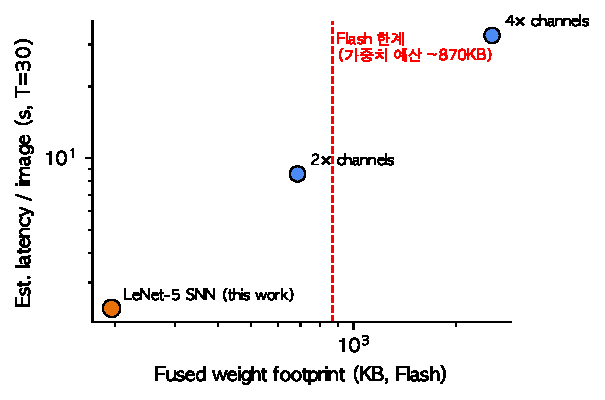
\includegraphics[width=0.86\linewidth]{figures/fig_envelope.pdf}
\caption{배포 가능 영역: 퓨전 가중치 Flash 용량 대 이미지당 추정
지연($T=30$, 양 축 로그). 수직 점선은 가중치 예산 약 870KB($=$1MB
$-$ 코드$\cdot$런타임 178.5KB)이며, 현 모델은 실측점,
2$\times$/4$\times$ 구성은 추정점이다.}
\label{fig:envelope}
\end{figure}

\subsection{타임스텝 축소 축}

지연의 또 다른 축은 $T$이다. 타임스텝당 시간이 일정하므로 지연은
$T$에 선형이고, $T=30\rightarrow10$이면 이미지당 약 0.8초로 추정된다.
학습 단계에서 관찰한 단일 이미지의 누적 스파이크 수렴 곡선은 판정이
$T<30$에서 조기 수렴할 수 있음을 시사하나, 이는 정성적 예시일 뿐이며
$T$ 축소에 따른 정확도 트레이드오프는 본 논문에서 검증하지 않았다.
